\documentclass[12pt,a4paper]{article}
\usepackage{setspace}
\usepackage{amsmath}			
\usepackage[utf8]{inputenc}		
\usepackage[T1]{fontenc}			
\usepackage[english]{babel}			
\usepackage{graphicx}			
\graphicspath{{images}}
\usepackage{subfigure}				
\usepackage{lscape}					
\usepackage{pst-plot, pstricks}		
\usepackage{fancybox,amssymb,color}	
\usepackage{setspace}				
\usepackage{booktabs}
\usepackage{longtable}	
\usepackage{adjustbox}	
\usepackage{multirow}		
\usepackage{float}	
\onehalfspacing
\pagestyle{plain}
\setlength{\parindent}{1em}
\setlength{\parskip}{1ex}
\usepackage[%  
colorlinks=true,
pdfborder={0 0 0},
linkcolor=black
]{hyperref}

\usepackage{geometry}   		 % definition of the page layout
\geometry{
	a4paper,					 % format
	left=25mm,					 % left margin
	right=25mm,					 % right margin
	top=25mm,					 % distance upwards
	bottom=25mm,				 % distance downwards
	includehead,				 % distance from upwards till the page header
}

%\graphicspath{{Abbildungen/}} 	 % Name des Unterverzeichnisses für Abbildungen

% Setting for the enumerate environment. Replaces the sub numbering of alphabet with numbers 
\renewcommand{\theenumi}{\arabic{enumi}}
\renewcommand{\labelenumi}{\theenumi}
\renewcommand{\theenumii}{\arabic{enumii}}
\renewcommand{\labelenumii}{\theenumi.\theenumii}
\renewcommand{\theenumiii}{\arabic{enumiii}}
\renewcommand{\labelenumiii}{\theenumi.\theenumii.\theenumiii}
\renewcommand{\theenumiv}{\arabic{enumiv}}
\renewcommand{\labelenumiv}{\theenumi.\theenumii.\theenumiii.\theenumiv}


\begin{document}
\begin{titlepage}
	\begin{center}
		\vfill{
			\Large
			Universidad del Norte \\ 
			\large 
			Facultad de Humanidades y Ciencias Sociales - \\
			Departamento de Economía 
		}
		\vfill{		
			\large 
		(PR, Semestre 2022-30)
		}
		\vfill{
			\LARGE
			% -------------------------------------------------------------------------------------
			% Your topic
			A characterization of Colombian industries under Schumpeter's patterns of innovation \\
			% -------------------------------------------------------------------------------------
			\vspace{1cm}
			\Large
			% -------------------------------------------------------------------------------------
			\textbf{Progress Report}
			% -------------------------------------------------------------------------------------
		}

	\end{center}
	\vfill{
		\normalsize
		% -------------------------------------------------------------------------------------
		% Your personal information
		\flushleft
		\begin{tabular}{@{\qquad}ll}
			Course: & Taller de Investigación \\
			Course Professor: & Prof. Dr. Juan Perilla  \\
			Supervisor 1: & Prof. Dr. Jana Schmutzler \\
			Supervisor 2: & Prof. Dr. Werner Bönte \\
			Due Date:  & 27.09.2022 \\
			Name: & Juan Taborda	\\
			%Anschrift: & Musterstraße 24\\
			%		   & 1234 Buxtehude\\	
			E-Mail Address: & jtabordaj@uninorte.edu.co
		\end{tabular}
	}
	% -------------------------------------------------------------------------------------
\end{titlepage}
	
	
% ============================================================================================================================
% Lists
% ===========================================================================================================================
\pagenumbering{roman}
\tableofcontents \newpage
\listoffigures
\listoftables \newpage
\pagenumbering{arabic}
\setcounter{page}{1}


% ============================================================================================================================
% Main text
% ===========================================================================================================================

\section{Introduction and problem statement}
	
Who drives innovation within an industry? Is it a small firm, or an established one? Is it an incumbent business or a novel startup? According to mainstream economics, several factors influx. For example, which market structure prevails may concentrate or disperse efforts, the existence of fierce entry barriers could dis-incentivize novel ideas in favour of established paradigms, specialization in certain activities could place industries at the source of a supply chain and dedicate all its efforts in supplying other sectors, or patents could motivate cooperation and foster the appropriation of an invention’s gains. 

This article will answer this question using Joseph Schumpeter’s (1911;1942) Mark I and Mark II innovation patterns. Both archetypes assess a different market structure. While Mark I argues that novelty does not enter markets at the hand of incumbent firms but by entrant firms or new startups, Mark II appoints not the bold new enterprise or the brave startup but the large corporation as the driver of innovation. 

As with every theory, its importance relies on its results when tested empirically. Fontana et al. (2012) pointed out an untapped potential for Mark I and Mark II patterns in this field. Moreover, existing characterizations for both Marks have “\textit{been standing the test of time quite well}". There have been progress con characterizing industries with this pattern (Breschi et al., 2000; Castellaci and Zheng; 2010; Malerba and Orsenigo, 1996), which in turns gives a better insight of innovative activities in the countries where it takes place and serves as platform for policymakers to set up better guidelines for innovation-related policies. 

But Fontana et al. overlook the concentration of this type of studies across the globe. Even though there are contributions to fill this gap worldwide, assessments in some countries are missing, with emphasis on countries outside the global north and core economies such as Colombia.  

A gap in characterization eventually leads to a need for information. Hence, this document will employ information contained in DANE (2020) “\textit{Encuesta de Desarrollo e innovación tecnológica}” (EDIT) survey and DANE (2019) “\textit{Encuesta Anual Manufacturera}” (EAM) survey for manufacturers to characterize industries as Mark I or Mark II, according to their International Standard Industrial Classification code (ISIC, or CIIU in Spanish), emphasizing on Section C: Manufacturing. The EAM survey provides, with a yearly frequency, information on the manufacturing sector that allows a detailed understanding of its structure and evolution. EAM surveys hold variables related to sales, output, investment, export, number of employees, among others. 

On the other hand, the EDIT survey tackles the need for information about the type of innovative activities (radical or incremental), and their effects in firm performance such as cost reductions or productivity enhancements. Moreover, there is data about sources of financing, information usage, human capital qualities, usage of patents, copyright, and other non-conventional protection methods. According to the DANE (2020) methodological overview, the EDIT survey preserves a theoretical framework that welcomes most of the methodological guidelines of the Organization for Economic Cooperation and Development (OECD), with emphasis on its innovation-tailored OSLO Manual.  

This goal sets an intriguing task. First, there is novelty as earlier attempts to characterize all Colombian industries through Schumpeter patterns of innovation seem to be missing. Second, the characterization of industries yields useful information for future works and policymaking for one of the most important sectors in the country. Bear in mind that Colombian manufacturing has a 10\% share on its GDP (Gross Domestic Product), but accounting for aggregated value chains, it composes more than one-third of the economy (Arbelaez et al., 2021). 

\section{Objective Setup}
\begin{enumerate}
	\item \large Characterize industries in the Colombian manufacturing sector based on the framework of Schumpeter’s Mark I and II, aiming to supply a better insight on the differences between industries by finding out what type of firm drives innovation. 
\begin{enumerate}
	\item \normalsize Utilize information from the EDIT and EAM surveys to set up a database about firm features in manufacturing industries. 
	\item Based on EDIT and EAM information, construct a quantitative analysis at the firm level that yields a result at the industry level, which in turn gives groundwork to create industry-level comparisons. 
	\item Employing a cluster algorithm, group industry-level data by common patterns and characterize them using Schumpeter's Mark I and II, which will give an insight into the drivers of innovation constrained to industrial structure and dynamics.
\end{enumerate}
\end{enumerate}

\section{Theoretical Framework}

\textbf{The concept of innovation and its taxonomies }

The base of innovation-related studies is to set up the concept of innovation and innovative activities. According to the OECD (2018), innovation is a "\textit{New or improved product or process (or a combination thereof) that differs significantly from the unit's previous products or processes and that has been made available to potential users (product) or brought into use by the unit (process})" (p. 20).  

Although the OSLO manual points out that innovation is inherently subjective, its practical application is objective if we consider shared grounds for novelty, utility, and the capacity to evidence significant differences. In that sense, the OSLO manual defines innovative activities as "\textit{all developmental, financial and commercial activities undertaken by a firm that is intended to result in an innovation for the firm}" (p. 20). Despite being a firm-centric perspective, OECD's concept can also apply to markets and industries. Moreover, OECD nuances whether innovation tailors towards business practices, productive processes, goods, services, and marketing.  

Innovation may have two taxonomies based on its novelty and impact. The efforts of Schumpeter (1942) focused on the nature of radical innovations as departing from known opportunities looking to forge something new at the expense of destroying something old. Schumpeter perspective of innovation would create the concept of creative destruction. On the other hand, Kirzner (1973) argued that human alertness to new opportunities yields more rents when channelled into incremental innovations, those who do not compromise the\textit{ status quo} and work under the realm of known opportunities. 

In the case of the OSLO manual, two are identified. First, radical innovations, transform the\textit{ status quo.} The second, disruptive innovations, takes root in simple applications of niche markets and then diffuses throughout it; it does not immediately compromise the \textit{status quo}, but eventually displaces established firms (OECD, 2018, p. 78). For this research, we will employ the concepts of radical innovations as those that alter the\textit{ status quo} and have the potential to displace established firms, and incremental innovations as those that stem from improvements to existing ideas that do not alter the current paradigm of the market. \\

\noindent \textbf{Schumpeterian patterns of innovation }

It was not the OECD that introduced innovative patterns. It was Schumpeter (1911; 1942) who explored these differences and pioneered on the proposal of differentiated archetypes for innovation. In his 1911 book "The Theory of Economic Development", he employs a metaphor that sums up his early thoughts on how new combinations enter the market: "\textit{(…) in general it is not the owner of stagecoaches who builds railways}" (p. 66). The premise of Schumpeter implies that novelty does not enter the market at the hand of incumbent firms but by entrant firms. This idea would be coined as Schumpeter's Mark I, which places entrant firms as the drivers of innovation.  

Schumpeter's ideas would change later in his 1942 book "\textit{Capitalism, socialism and democracy": "(...) a shocking suspicion dawns upon us that big businesses may have had more to do with creating that standard of life than with keeping it down}" (p. 82). Such perspective departs from Mark I and will become Schumpeter's Mark II. In contrary to a Mark I market, Schumpeter appoints large, established firms as the driver of innovation. It is not the bold new enterprise or the brave startup that brings new goods or services but the tried and true stable, large corporation. Schumpeter would reinforce Mark II thereon in the book: "\textit{Perfect competition is not only impossible but inferior and has no title to being set up as a model of ideal efficiency}" (p. 106). \\

\noindent \textbf{Market structure and innovation }

Mark I and II may seem exclusive. They are not \textit{per se}, but the subjacent market structures they assess. According to Fontana et al. (2012), one may classify industries using Mark I and Mark II archetypes. Mark I industries are turbulent, with low entry barriers and fiercer competition. On the other hand, stable environments with large established firms and entry barriers characterize Mark II industries. In other terms, Schumpeter's Mark I and Mark II concede the existence of two fundamental market structures bonded to the concept of innovation. Mark I approach perfect competition, while Mark II appeals to a monopolistic (or oligopolistic) structure. 

With an established framework using Schumpeter's contributions we can now add up its patterns with OECD's taxonomy. Considering Gilbert (2006) statement that the incentive to innovate is the difference in profits that a firm can earn if it decides to do so, which, according to Arrow (1962), is higher in perfect competition than in monopoly, because the existing monopoly power acts as a formidable disincentive to innovate, then perfect competition seems to have the suitable incentives to introduce breakthroughs in the market. Baumol (2004) reinforces this idea by saying: “\textit{major breakthroughs have tended to come from small new enterprises}” (p. 10). In that sense, risky innovations that seek to disrupt the \textit{status quo}, which OECD labels as radical innovations, seem to relate to perfect competition structures, which appeals to a Mark I pattern.  

Baumol (2004) observation continues: “\textit{(…) while the invaluable incremental contributions that multiply capacity and speed and increase reliability and user-friendliness have been the domain of the larger firms}” (p. 10). This allows us to construct the definition of the market structure related to OECD incremental innovations taxonomy. By considering Arrow’s replacement effect and Gilbert statement on innovation incentives, we have strong signals that incremental innovations suit concentrated markets. Surely, entry barriers and high endowments of resources supply a deterrence to potential entrants, but when it comes to innovation, monopolies have less incentives to change the paradigm of their markets, as they can compromise existing gains. Therefore, incremental enhancements, as Baumol exemplifies, that increase reliability or user friendliness, characterize concentrated markets. In this case, the innovation pattern appeals to Mark II.  

As an overlook of both Schumpeter’s and Arrow’s theories, Shapiro (2012) remarks that the unifying principle of both is that a contestable market and potential profits from sales spur innovation. Moreover, a firm that wants to maintain the \textit{status quo} (I.e., Monopolies) has a smaller incentive than new entrants (let it be, a small startup) to disrupts said status by introducing radical innovations. 

\section{Literature Review}

A first prominent characterization exercise comes from Malerba and Orsenigo (1996), who identified Schumpeter’s Mark I and Mark II across 49 technological classes of six countries: the US, Japan, Germany, France, the UK, and Italy. The authors find Mark I as a widening pattern, where concentration of innovative activities is low, with small sized firms and low stability in the ranking of innovations. On the other hand, they find Mark II as a deepening pattern: high market concentration, larger firms, a stable ranking of innovators and deterrents to entry. 

Further contributions by Breschi et al. (2000) suggest that better appropriability conditions work in the direction of Schumpeter’s Mark II patter, while the opposite appeals to Schumpeter’s Mark I. Their contributions do align with earlier results by Malerba and Orsenigo, reinforcing their findings. By principal component analysis, they found that the ability to employ protection mechanisms to protect innovation has a positive relation with Schumpeter Mark II. Moreover, low market concentration reinforces widening patterns (Mark I), and high stability appeals to Mark II.   

Fontana et al. (2012) connects with Breschi et al. (2000) contributions. Moreover, Landström \& Schön (2010) not only report similar findings, but also remark on similarities between patterns. For example, innovation is central to economic development and in both the capitalist assumes the risk.  

However, Schumpeter marks are not alone in the literature. around the eighties, a new set of archetypes by Pavitt (1984) proposed an alternative to Schumpeter’s Mark I and Mark II. Pavitt's (1984) taxonomy classifies industries based on the requirements of its users, the sources of its technologies, and the degree of appropriability. Pavitt finds four different patterns for industries: Supplier-dominated sectors; scale-intensive industries employing process and product innovation; specialized suppliers that market technology to other firms; finally, science-based, knowledge industries with a high degree of appropriability and tailored towards exploring innovative technological breakthroughs.  

One may ask which framework is better. However, both appeal to distinct aspects of the same subject. In the case of Pavitt’s taxonomy, Archibugi (2001) finds that each one closely ties with Kondratiev's long waves of capitalist development. On the other hand, Castellacci (2008) links its classification to the sectors that sustained the growth of advanced economies in the Fordist age. In contrast, Schumpeter's Mark I and II appeal to the dynamics of an industry life cycle. Mark I characterize the early stage of a firm, where turbulence in competition is common and there is no clear leader. On the other hand, Mark II refers to a more mature, late-stage phase of an industry that has large firms deeply rooted on the market (Malerba, 2005).

The question revolves not around which framework is better but on when and how to use these frameworks. In the literature, authors like Fontana et al. (2021), Breschi et al. (2000), Castellaci and Zheng (2010), Malerba and Orsenigo (1996), Corrocher et al. (2007), among others focused their efforts on Schumpeter's patterns. In contrast, Landström \& Schön (2010), Marsili and Verspagen (2002), and Leiponen and Drejer (2007) preferred an approach using Pavitt's taxonomy.  

The selection of either Schumpeter’s or Pavitt’s framework relies usually on the scope and objectives of the research. For example, Breschi et al. (2000) wanted to test Schumpeter’s hypotheses through quantitative analysis, Corrocher et al. (2007) aimed to create a distinction for ICT sectors based on Schumpeter’s work, proving a coexistence of both Marks in some cases, and Castellaci and Zheng (2010) deployed an industry-level productivity growth characterization using Schumpeterian patterns. However, the literature has found that sometimes Schumpeter’s pattern may offer a narrow view of an industry, which makes them employ Pavitt’s taxonomy. Such is the case of Van Dijk (2000), who showed how some groups among Dutch manufacture do not fit easily into either group of Schumpeter’s Marks, or Leiponen and Drejer (2007) with a similar phenomenon on Danish industries. 

Characterizing exercises yields information on how their industries work and what environment they enclose. Policymaking can borrow elements from these studies. However, as we stated previously, tension builds in countries or regions where this exercise does not exist. With the emphasis on Colombia, Schumpeter's theory is known, as some articles appeal to its contributions to their study (Umaña-Aponte et al., 2013; Marroquín, 2010; Arroyo-Mina \& Guerrero, 2018; Langebaek-Rueda \& Vásquez, 2007). Nonetheless, it is not used for characterization of industries but for impact evaluation, behavioral economics, and case analysis.  

There are attempts to build sector-specific entrepreneurship profiles (Cerón et al. 2010), and innovative profiles (Ovallos-Gazabón \& Amar-Sepúlveda, 2014), but they do not employ Schumpeterian patterns of innovation. With that in mind, this article will join the academic dialogue about innovation patterns in Colombia by characterizing industries in the manufacturing sector. I intend to reach this goal by characterization Colombian manufacturing industries using Schumpeter's framework, which will supply insight into how firms behave toward innovation, based on industrial life cycle and dynamics. 

\section{Methodology}

This research employs a cross-section hybrid of DANE (2020) “\textit{Encuesta de Desarrollo e innovación tecnológica}” (EDIT) survey and DANE (2019) “\textit{Encuesta Anual Manufacturera}” (EAM) survey. Both surveys differentiate firms by a “\textit{Numero de Orden}” (NORDEMP) registration, which makes it easier to identify common patterns and merge them in one single database.  

EAM is a census of all manufacturing industries in Colombia that fulfils its classification criterion of at least ten employees and sales greater than 517 million pesos. If a firm fulfil the sales requirement but not the employees one, it is also included in the census. This implies that the EAM by itself is a population database, not a sample. Moreover, given the sales and employment thresholds, the informal economy, small and micro firms end up excluded from the survey. As Annex 1 illustrates, the selection at the four-level ISIC digits is based on the following three digits industries \footnote{Source: Own elaboration based on DANE's Methodology (2018, p. 7)}\footnote{As an exception, ISIC codes 202 and 210 select specific four-digit industries within them}. 

Given the fact that EDIT samples EAM sectors, instead of firms, not every industry in EAM is present in the EDIT. By using statistical software like R, I solve this problem through an inner join of both databases by their common ISIC code and NORDEMP registrations. Thus, the yielding database reduced the number of observations from almost 8000 to 6405. 

From this database, I will employ some of the variables that approach Breschi et al. (2000), and Malerba \& Orsenigo (1996) dimensions: market concentration, stability and technological opportunities, an. Based on these dimensions the relevant variables found on the EDIT/EAM cross are: 

\begin{table}[h!]
	\centering
	\caption{Relevant variables for the study}
	\begin{tabular}{lcl}
		\hline
		\multicolumn{1}{c}{\textbf{Dimension}}                                                  & \textbf{Concepts}                                                                                                                                           & \multicolumn{1}{c}{\textbf{Variables (by   DANE's code)}} \\ \hline
		\multirow{2}{*}{Stability}                                                              & \begin{tabular}[c]{@{}c@{}}Amount of \\ radical innovations\end{tabular}                                                                                    & I1R4C2N                                                   \\ \cline{2-3} 
		& \begin{tabular}[c]{@{}c@{}}Amount of\\  incremental innovations\end{tabular}                                                                                & I1R4C2M                                                   \\ \hline
		\multirow{4}{*}{Concentration}                                                          & Total sales                                                                                                                                                 & I3R2C1                                                    \\ \cline{2-3} 
		& \begin{tabular}[c]{@{}c@{}}Total spending on \\ innovative activities\end{tabular}                                                                          & II1R10C2                                                  \\ \cline{2-3} 
		& Total Employees                                                                                                                                             & PERTOTAL                                                  \\ \cline{2-3} 
		& Total Output                                                                                                                                                & PRODBIND                                                  \\ \hline
		\multirow{3}{*}{\begin{tabular}[c]{@{}l@{}}Technological \\ Opportunities\end{tabular}} & \begin{tabular}[c]{@{}c@{}}Possession of conventional \\ protection mechanisms \\ valid until 2018 (Patents, \\ IP,  Copyright, \\ Trademarks)\end{tabular} & VI1R8C2                                                   \\ \cline{2-3} 
		& \begin{tabular}[c]{@{}c@{}}Obtention of conventional \\ protection mechanisms \\  between 2017-2018\end{tabular}                                            & VI2R8C2                                                   \\ \cline{2-3} 
		& \begin{tabular}[c]{@{}c@{}}Usage of non-conventional \\ protection mechanisms\\  (NDA, \\ industrial secrets, \\ high complexity on designs)\end{tabular}   & VI3R5C2                                                   \\ \hline
	\end{tabular}
		Source: Own elaboration based on DANE’s surveys (2019;2020)
\end{table}

By making use of these variables in R, I construct 3 dimensions at the industry level: Concentration (\textit{CON}), Technological Opportunities (\textit{TO}) and Stability (\textit{STA}). The way to measure these variables adopts the following forms: 

\begin{enumerate}
	\item \textit{CON}: Based on the works of Malerba and Orsenigo (1996), it is a measure of concentration of innovative activities and firm size. At the firm level, I employ these variables, but also extend the measure to include market share in number of employees and total output. Variations between these shares are smoothened by using a geometrical mean such that the industry-level measure adopts the form: 
		\begin{equation}
			\centering
			CON = (HH_{ms}*HH_{msa}*HH_{lsd}*HH_{ss})^{1/4}
		\end{equation}
	Where $HH$ is a Herfindahl-Hirschman index, and the subindex represent each measure of interest. In that sense, $ms$ means Market Share, $msa$ means Innovative Activities, $lds$ stands for Labour Demand Share, and $ss$ for Supply Share. Per our established conceptual review, we expect that low values of the \textit{CON} measure will relate to Mark I industries, while large coefficients would appeal to Mark II industries. 
	\item \textit{TO}: I employ Maleki et al. (2018) approach, where Technological Opportunities are measured by the growth rate of patents. However, growth rate requires a comparable measure for 2017. I do not possess this data as EDIT surveys are non-comparable. Thus, I employ the proportion of new protection mechanism relative to registered mechanisms. In this case, we can employ the following formula at the industry level: 
	\begin{equation}
		\centering
		TO = \dfrac{PM_{1718} + NCPM_{1718}}{PM}
	\end{equation}
	Where $PM_{1718}$ captures the industry aggregate of all protection mechanisms obtained between 2017 and 2018, $NCPM_{1718}$ follows the same mechanism, but with emphasis on non-conventional protection mechanisms (e.g., Non-Disclosure Agreements, Industrial Secrets and Complex Design). Finally, $PM$ contains all protection mechanisms valid until the end of the year of interest (2018). Considering Breschi et al (2000) distinction, Mark I industries have low appropriability for their inventions, while Mark II tend to appropriate knowledge better and possess more technological opportunities. Thus, we may speculate in favour of an inclination towards Mark II on industries with high TO values. 
	\item \textit{STA}: Since stability has close ties with firms entering and exiting the market of innovation, it demands a dynamic analysis. Bear in mind that DANE’s EDIT methodology states that EDIT 2018 is non-comparable with its predecessors. Thus, we need to employ a different approach.  
	
	To solve this setback, I borrow theoretical concepts from the literature. Specifically, I rely on Baumol (2004, p. 10) observation that “\textit{major breakthroughs have tended to come from small new enterprises, while the invaluable incremental contributions (…) have been the domain of the larger firms}.”. Baumol proposition, coupled with the relationship between firm size and Schumpeterian patterns established in the literature review, provides a stability approach that could be classified under either Mark I or II. Hence, to quantify that stability approach, I propose the following mathematical form: 
	\begin{equation}
		\centering
		STA = Sr - Si
	\end{equation}
Where $Sr$ is the share of radical innovations over the total amount of innovations in the industry, and $Si$ the share of incremental innovations. Based on Baumol’s proposition and reviewed theory, we shall expect a high share of radical innovations to have a relation with turbulent Mark I industries, while incremental innovations to the Mark II archetype. 
\end{enumerate}

Considering the nature of these three dimensions, I had to filter the database further, as some industries, for example, reported an aggregate of zero on innovation activities spending. Therefore, the concentration measure would result in zero, even though the other components do report values greater than zero. This began to be a problem on industries with less than 20 observations. Hence, I establish 20 as the minimum number of observations in my study. Results are reported on Annex 2.

The information is then clustered using a k-means method for 2 groups, employing a Lloyd algorithm and 10 repetitions. Following MacKay (2003) explanation, k-means calculates a mean for each group and assigns a data point (in this case, industry) to said group by the following mechanism: 

\begin{enumerate}
	\item \textit{Assignation phase}: Each observation gets assigned to the group with the closest mean (by Euclidean distance). Each generated group is composed by a centroid that serves as reference point for the following steps.  
	\item \textit{Update phase}: Group parameters adjust to match the means of the data points. 
	\item \textit{Repetition phase}: Assignation and Update phases repeat until they do not change anymore, that is, data points do not change their position in the groups. 
\end{enumerate}

\section{The Cluster}
\subsection{Preliminary Results}
\begin{figure}[H]	
	\caption{Preliminary characterization of Colombian Manufacture using a two groups k-means clustering method}
	\centering
	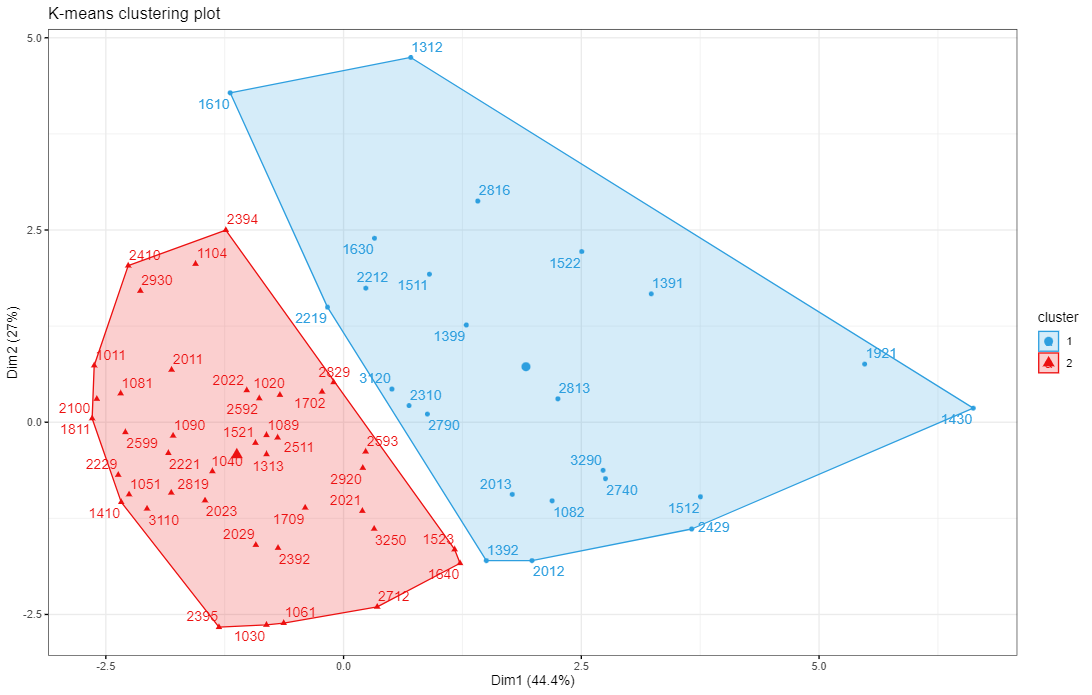
\includegraphics[scale = 0.45]{cluster.png}
	Source: Own elaboration based on DANE (2019;2020) databases.
\end{figure}

Figure 1 shows the resulting cluster from the k-means algorithm. Before evaluating both groups, bear in mind that the X and Y axis are in function of “Dim1” and “Dim2” variables, instead of our initial measures. This change obeys to the fact that the k-cluster method in R employs a principal component analysis (PCA) dimensional reduction algorithm. PCA operates our three dimensions (\textit{STA, TO, CON}) and creates “shadow” variables "Dim1" and "Dim2". These variables capture a certain amount of the variation contained in the original dataset. In this case, Dim1 and Dim2 find components of 44.4\% and 27\% respectively. 

In our 2 groups k-means clustering exercise, we find that Cluster Group 2 (CG2), colored red, has 5192 observations and is denser than Cluster Group 1 (CG1), colored blue, which has 794 observations. On the other hand, red group industries are closer between them than those in the blue group. Initial descriptive statistics for both groups are shown in the following table. 

\begin{table}[h!] 
	\caption{Initial descriptive statistics of the two groups k-means clustering}
	\centering
	\begin{tabular}{@{}lllllll@{}} 
		\toprule 
		\multicolumn{1}{c}{} & \multicolumn{3}{c}{\textit{Cluster Group 2}}                   & \multicolumn{3}{c}{\textit{Cluster   Group 1}} \\ \midrule 
		
		& \textit{TO} & \textit{CON} & \multicolumn{1}{l|}{\textit{STA}} & \textit{TO}   & \textit{CON}   & \textit{STA}  \\ \cmidrule(l){2-7}  
		
		\textit{Max}         & 3.500       & 1023.11      & \multicolumn{1}{l|}{0.586}        & 6.000         & 2702.96        & 1.000         \\ 
		
		\textit{Min}         & 0      & 160.28       & \multicolumn{1}{l|}{-1.000}       & 0.047        & 1068.11        & -1.000        \\ 
		
		\textit{Mean}        & 0.522      & 572.22       & \multicolumn{1}{l|}{-0.294}       & 0.983        & 1507.72        & -0.345        \\ 
		
		\textit{Std Dev}     & 0.651       & 262.98       & \multicolumn{1}{l|}{0.414}        & 1.496         & 416.08         & 0.550         \\ \bottomrule 
	\end{tabular} \\ 
 	Source: Own elaboration 
\end{table} 

Initial differences arise on the preliminary descriptive statistics, which may aid in our characterization purpose. In the case of CG2, Technological Opportunities oscillate between a growth rate of 350\% and no growth at all, with a representative value of 0.52 and a standard deviation of 0.65. Concentration values in CG2 tend to be smaller, oscillating between 1023 and 160 on the Herfindahl-Hirschman index and reporting a representative value of 1507. Standard deviation across concentration stands at 262 index points. Finally, Stability reports values between 0.586 and –1 with a standard deviation of 0.414 and a mean of –0.294 

In the case of CG1, we find a large value of Technological Opportunities, with industries reporting a growth rate of 600\% relative to existing protection mechanisms. The mean of this group stands near 1 with a standard deviation of 1.496, telling us about an overall feature in this group to grow their protection mechanism registries more than their CG2 counterparts. Concentration index in CG2 also reports a significant deviation from CG1 results. While the former oscillates between 2702 and 1068, with a representative value of 1507, the latter passes maximum 1000 index points. Finally, Stability reports in average slightly higher values towards incremental innovations when compared to CG1.  

\subsection{Preliminary Analysis}

In this section, I put the results in context with Schumpeterian patterns of innovation by employing further data visualization and inferences. To begin with, results report lower Stability in CG2 when compared to CG1. Even though the mean difference fin both groups is not large, data distribution as per the Figure 2 shows that the density plot for CG1 has a prominent number of observations between 0 and -1, which in turn means, by the nature of the measure employed, that CG1 has many industries with a predominance of incremental innovations in their aggregates. This remark is reinforced by a high positive skew of the distribution. 

In the case of CG2, the next figure shows that it distributes mostly below 0, but its differentiating factor is its lower density when compared to CG1 across said interval. Skewness and kurtosis measures support this idea. The main insight to draw from this analysis is that CG1 industries tend to be dominated by larger shares of incremental innovations in their aggregate, while industries in CG2 do not show this tendency, instead, they have smaller differences between radical and incremental shares rather than disproportions towards one of the two types. Box plots support this conclusion, considering that CG1 left box is much wider than its CG2 equivalent.

\begin{figure}[H]	
	\caption{Density and box plots of both Groups in the Stability dimension.}
	\centering
	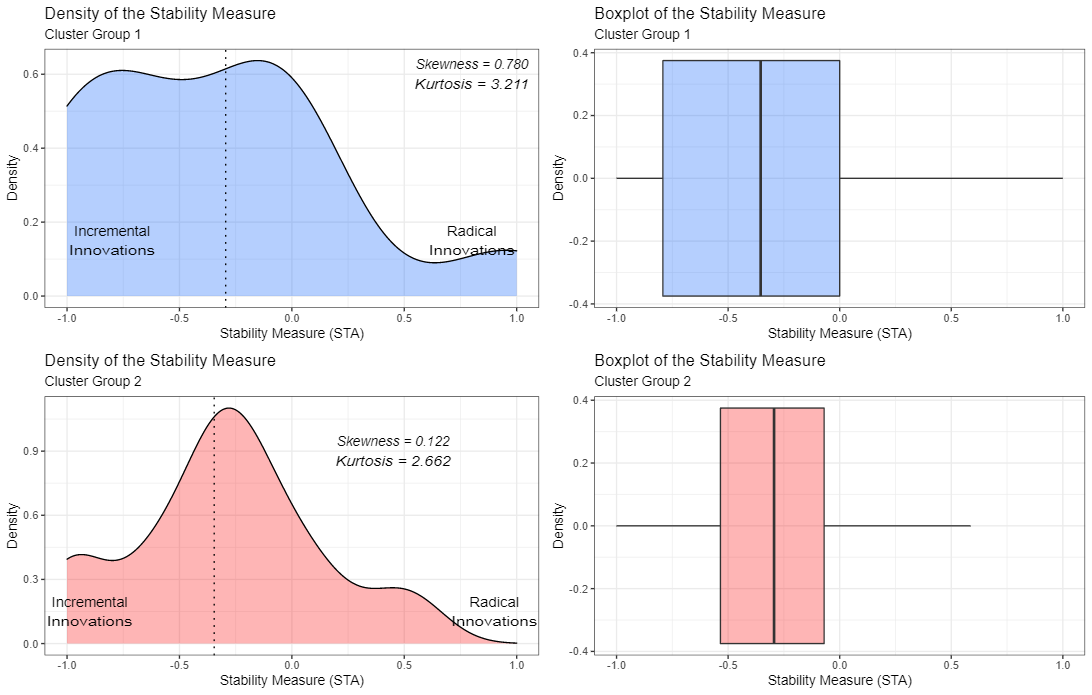
\includegraphics[scale = 0.45]{sta.png}
		Source: Own elaboration
\end{figure}

Within the Concentration measure, density plots in the next figure show a clear difference between both groups.  While CG2 distribution finds its peak near 500 and reaches 1000 concentration points at most, CG1 reports values above 1000, with a long-tailed right side until 2700. Boxplot of both datasets provides a different visualization of this phenomenon, but confirms that CG1 market concentration is, on average, much larger than industries on CG2. All this statistical insight points out to one conclusion: CG1 industries are highly concentrated, and, dominated by larger firms. 

\begin{figure}[H]	
	\caption{Density and box plots of both Groups in the Concentration dimension.}
	\centering
	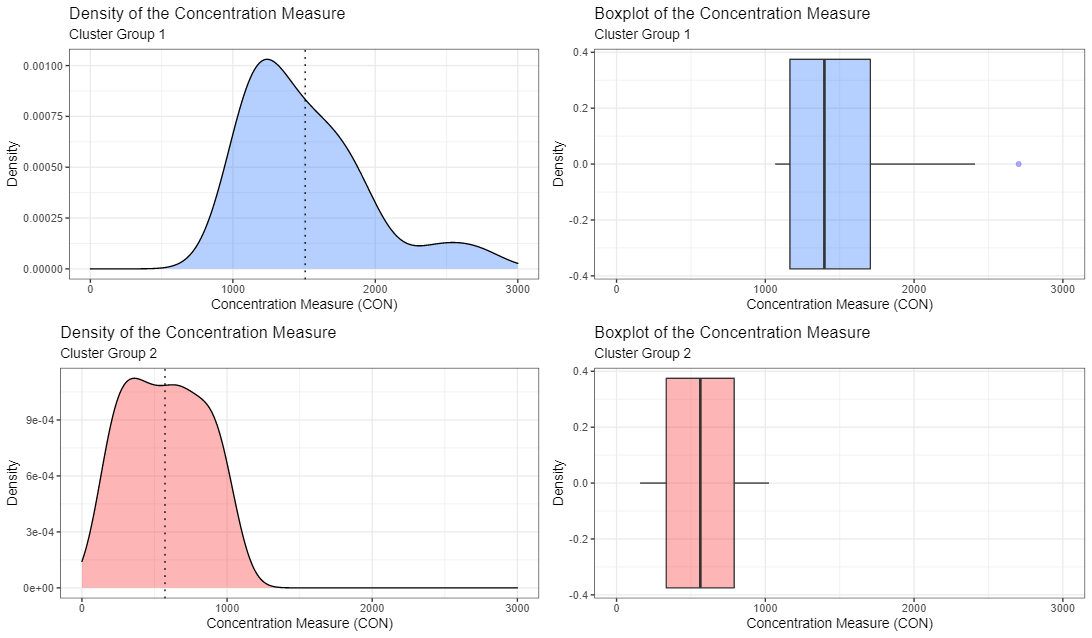
\includegraphics[scale = 0.45]{pcon.png}
		Source: Own elaboration
\end{figure}

Finally, the behaviour of technological opportunities shows that both groups distribute mostly near zero. However, as shown in the next figure, skewness in CG2 is larger than CG1, which may lead us to infer that their registry of new protection mechanisms relative to the existing ones is low, which in turn may indicate low appropriability. Kurtosis in CG2 is also higher, which indicates that the TO measure industries classified on CG2 is highly concentrated around its mean. In the case of CG1, both moments are lower. Thus, CG1 industries do register a higher proportion of protection mechanisms relative to the existing ones compared to CG2, which may indicate an overall higher level of appropriability in this group. Box plots reinforce this idea, as CG1 right box is wider. 

\begin{figure}[H]	
	\caption{Density and box plots of both Groups in the Technological Opportunities dimension.}
	\centering
	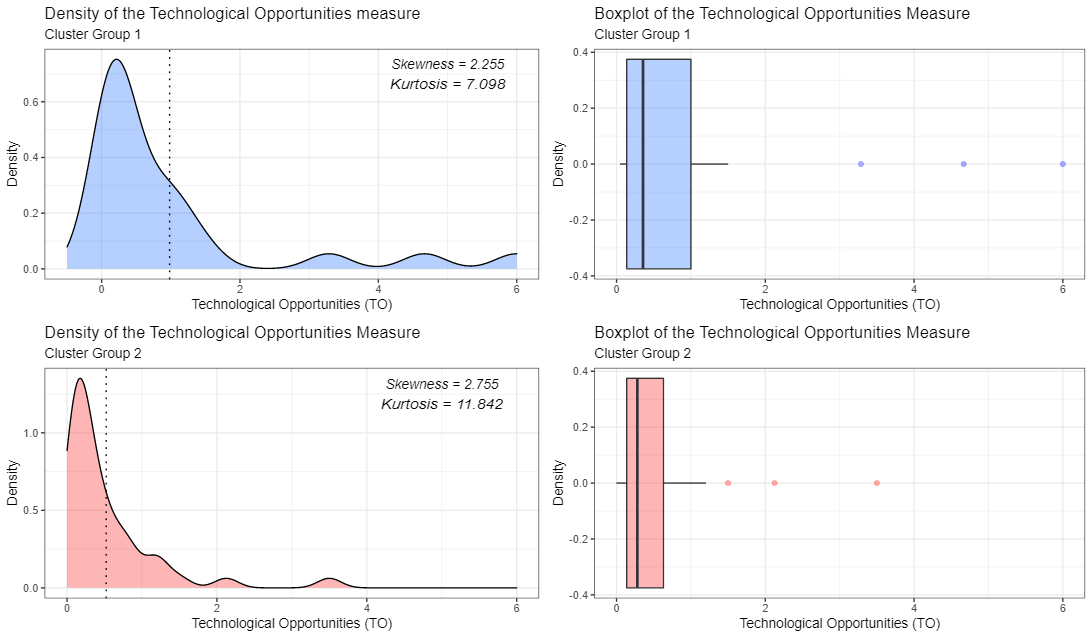
\includegraphics[scale = 0.45]{to.png}
		Source: Own elaboration
\end{figure}

By evaluating these three dimensions, let us go over again our most important discoveries. First, we found a tendency in CG1 towards high shares of incremental innovations, while CG2 tends to be more balanced between shares. Second, CG1 market concentration is clearly larger in average than CG2, which in turn gives us reasons to argue in favour of large firms as the dominant agents of these industries. Finally, we found that CG1 industries register more protection mechanisms relative to the existing ones compared to CG2, which appeals to higher levels of appropriability as there are formal methods to secure benefits from innovation (I.e., Patents, IPs, Copyrights, et cetera). 

Per this inferential analysis, and based on reviewed theory, we can provide a preliminary characterization of CG1 industries under the Mark II pattern, while features of CG2 industries gravitate towards the Mark I Archetype.  

\section{Preliminary Conclusions}

Our preliminary conclusions revolve around three ideas. First, we have been able to characterize Colombian industries under Schumpeterian patterns of innovation. Even without the dynamic component of previous characterization exercises, statistical analysis and inference show clear differences, proper of Schumpeterian patterns.  

Second, we found what type of firm drives innovation on each industry. CG1, the less dense group, has been labeled as Mark II, thus, larger firms drive innovation within this group. On the other hand, CG2, the densest group, gravitates toward Mark I, placing startups and small firms as the drivers of I innovation. This difference in amount shows us that Colombian manufacture is more of a Mark I than Mark II sector, as the largest group of industries is the Mark I group.  

Third, concentration is the spearhead of innovation pattern analysis in Colombia, as the most prominent differences came from its measure. It is true that the Stability and Technological Opportunities measures yielded relevant results, but its analysis required further statistical tools to produce a formidable conclusion. 

Besides our data-driven conclusions, this characterization exercise provides an input for future works and serves as a groundwork for public policy recommendations. In the former, as every industry is now classified under a Schumpeterian pattern of innovation, it may serve as the starting point for a probabilistic exercise, in the latter, as we found who drives innovation within each industry, it may aid in future policies or reforms that tackle, for example, innovative activities or research incentives. 

\section*{References}
\emergencystretch 5em
\raggedright
{\setlength{\parindent}{-1.7em}
	\-\footnotesize.
	\normalsize
	
	Arbeláez, M. A., Becerra, A., \& Benítez, M. (2021). Contribución fiscal y tributación efectiva de la industria manufacturera en Colombia. http://www.repository.fedesarrollo.org.co/handle/11445/4071
	
	Archibugi, D. (2001). Pavitt’S Taxonomy Sixteen Years On: A Review Article. Economics of Innovation and New Technology, 10(5), 415–425. https://doi.org/10.1080/10438590100000016
	
	Arrow, K. (1962). Economic Welfare and the Allocation of Resources for Invention. En The Rate and Direction of Inventive Activity: Economic and Social Factors (pp. 609–626). Princeton University Press. https://www.nber.org/books-and-chapters/rate-and-direction-inventive-activity-economic-and-social-factors/economic-welfare-and-allocation-resources-invention
	
	Arroyo-Mina, J. S., \& Guerrero, D. (2018). Schumpeterian Behavior in a CPR Game: Experimental Evidence from Colombian Fisheries Under TURF’s Management. Mediterranean Journal of Social Sciences, 9(4), 109.
	
	Baumol, W. J. (2004). Entrepreneurial Enterprises, Large Established Firms and Other Components of the Free-Market Growth Machine. Small Business Economics, 23(1), 9–21. https://doi.org/10.1023/B:SBEJ.0000026057.47641.a6
	
	Breschi, S., Malerba, F., \& Orsenigo, L. (2000). Technological Regimes and Schumpeterian Patterns of Innovation. The Economic Journal, 110(463), 388–410. https://doi.org/10.1111/1468-0297.00530
	
	Castellacci, F. (2008). Technological paradigms, regimes and trajectories: Manufacturing and service industries in a new taxonomy of sectoral patterns of innovation. Research Policy, 37(6–7), 978–994. https://doi.org/10.1016/j.respol.2008.03.011
	
	Castellacci, F., \& Zheng, J. (2010). Technological regimes, Schumpeterian patterns of innovation and firm-level productivity growth. Industrial and Corporate Change, 19(6), 1829–1865. https://doi.org/10.1093/icc/dtq051
	
	Cerón, C. A., Alcazar, F. L., \& M, J. J. G. (2010). Caracterización emprendedora de los empresarios en los Valles de Tundama y Sugamuxi. Boyacá (Colombia). Pensamiento \& Gestión, 29, 163–189.
	
	Corrocher, N., Malerba, F., \& Montobbio, F. (2007). Schumpeterian patterns of innovative activity in the ICT field. Research Policy, 36(3), 418–432. https://doi.org/10.1016/j.respol.2007.01.002
	
	Departamento Administrativo Nacional de Estadistica DANE. (2019). Encuesta Anual Manufacturera – EAM - 2018. https://microdatos.dane.gov.co/index.php/catalog/650/study-description
	
	Departamento Administrativo Nacional de Estadistica DANE. (2020). Encuesta de Desarrollo e Innovación Tecnológica—EDIT - Industria—2017—2018 [Government Online Site]. https://microdatos.dane.gov.co/index.php/catalog/651/datafile/F38
	
	Departamento Administrativo Nacional de Estadistica DANE \& Dirección de Metodología y Producción Estadística. (2018). Metodología General Encuesta de Desarrollo e Innovación Tecnológica en la industria manufacturera—EDIT [Online government site]. DANE. https://microdatos.dane.gov.co/catalog/651/related\_materials
	
	Fontana, R., Martinelli, A., \& Nuvolari, A. (2021). Regimes reloaded! A reappraisal of Schumpeterian patterns of innovation, 1977–2011. Journal of Evolutionary Economics, 31(5), 1495–1519. https://doi.org/10.1007/s00191-021-00735-6
	
	Fontana, R., Nuvolari, A., Shimizu, H., \& Vezzulli, A. (2012). Schumpeterian patterns of innovation and the sources of breakthrough inventions: Evidence from a data-set of R\&D awards. Journal of Evolutionary Economics, 22(4), 785–810. https://doi.org/10.1007/s00191-012-0287-z
	
	Gilbert, R. (2006). Looking for Mr. Schumpeter: Where Are We in the Competition--Innovation Debate? Innovation Policy and the Economy, 6, 159–215.
	
	Kirzner, I. M. (1978). Competition and Entrepreneurship. University of Chicago Press. https://press.uchicago.edu/ucp/books/book/chicago/C/bo27304815.html
	
	Landström, H., \& Schön, L. (2010). Industrial Renewal and Entrepreneurship in Sweden: A Structural Cycle Explanation. Historical Foundations of Entrepreneurship Research. https://www.elgaronline.com/view/edcoll/9781847209191/9781847209191.00029.xml
	
	Langebaek-Rueda, A., \& Vásquez, D. M. (2007). Determinantes de la actividad innovadora en la industria manufacturera colombiana. Banco de la República. https://doi.org/10.32468/be.433
	
	Leiponen, A., \& Drejer, I. (2007). What exactly are technological regimes?: Intra-industry heterogeneity in the organization of innovation activities. Research Policy, 36(8), 1221–1238. https://doi.org/10.1016/j.respol.2007.04.008
	
	MacKay, D. J. C. (2003). Information theory, inference, and learning algorithms. Cambridge University Press.
	
	Maleki, A., Rosiello, A., \& Wield, D. (2018). The effect of the dynamics of knowledge base complexity on Schumpeterian patterns of innovation: The upstream petroleum industry. R\&D Management, 48(4), 379–393. https://doi.org/10.1111/radm.12251
	
	Malerba, F. (2005). Sectoral systems of innovation: A framework for linking innovation to the knowledge base, structure and dynamics of sectors. Economics of Innovation and New Technology, 14(1–2), 63–82. https://doi.org/10.1080/1043859042000228688
	
	Malerba, F., \& Orsenigo, L. (1996). Schumpeterian patterns of innovation are technology-specific. Research Policy, 25(3), 451–478. https://doi.org/10.1016/0048-7333(95)00840-3
	
	Marroquín, G. A. (2010). Is Joseph Schumpeter’s theory of economic development still useful? The case of a semirural community in Colombia. En D. C. Wood (Ed.), Economic Action in Theory and Practice: Anthropological Investigations (Vol. 30, pp. 77–98). Emerald Group Publishing Limited. https://doi.org/10.1108/S0190-1281(2010)0000030007
	
	Marsili, O., \& Verspagen, B. (2002). Technology and the dynamics of industrial structures: An empirical mapping of Dutch manufacturing. Industrial and Corporate Change, 11(4), 791–815. https://doi.org/10.1093/icc/11.4.791
	
	OECD \& Eurostat. (2018). Oslo Manual 2018: Guidelines for Collecting, Reporting and Using Data on Innovation (4th ed.). OECD Publishing. https://www.oecd-ilibrary.org/science-and-technology/oslo-manual-2018\_9789264304604-en;jsessionid=82Pf8iyig0VUix25LgMRN\_ka.ip-10-240-5-20
	
	Ovallos-Gazabón, D. A., \& Amar-Sepúlveda, P. A. (2014). Perfil innovador de la industria manufacturera colombiana. Caso del sector metalmecánico de Barranquilla. Revista Ingenierías Universidad de Medellín, 13(25), 115–136. https://doi.org/10.22395/rium.v13n25a8
	
	Pavitt, K. (1984). Sectoral patterns of technical change: Towards a taxonomy and a theory. Research Policy, 13(6), 343–373. https://doi.org/10.1016/0048-7333(84)90018-0
	
	Schumpeter, J. (1911). Theory of Economic Development (1a ed.).
	
	Schumpeter, J. A. (1942). Capitalism, Socialism and Democracy. Routledge.
	
	Shapiro, C. (2012). Competition and Innovation Did Arrow Hit the Bull’s Eye? En The Rate and Direction of Inventive Activity Revisited (pp. 361–410). University of Chicago Press. https://doi.org/10.7208/chicago/9780226473062.001.0001
	
	Umaña-Aponte, M., Estupiñan, F., \& Duque, C. (2013). Innovation and productivity in services: An impact evaluation of Colciencias funding programs in Colombia [Working Paper]. Centro de Investigaciones Económicas (CINVE), Montevideo, UY. https://doi.org/10/DT-N\%C2\%B0-2013\_SS-IP\_-08-METRICA.pdf
	
	van Dijk, M. (2000). Technological regimes and industrial dynamics: The evidence from Dutch manufacturing. Industrial and Corporate Change, 9(2), 173–194. https://doi.org/10.1093/icc/9.2.173
	


\pagebreak
\newpage
\appendix
\section{Annex 1: Universe of study for the EDIT survey.}

\begin{longtable}{@{}lc@{}}
	\toprule
	\multicolumn{1}{c}{\textbf{ISIC code}} & \textbf{Economic   activity}                                             \\ \midrule
	101                                            & Processing   and preservation of meat and fish                           \\
	102                                            & Processing and preservation of   fruits, vegetables and tubers           \\
	103                                            & Production of oils and fats                                              \\
	104                                            & Dairy Processing                                                         \\
	105                                            & Production of milling products,   starches and their derivatives         \\
	106                                            & Elaboration of coffee products                                           \\
	107                                            & Sugar and panela processing                                              \\
	108                                            & Manufacture of other foodstuffs                                          \\
	109                                            & Preparation of prepared   feedingstufss for animals                      \\
	110                                            & Beverage production                                                      \\
	131                                            & Spinning, weaving and finishing   of textiles                            \\
	139                                            & Manufacture of other textiles                                            \\
	141                                            & Manufacture of clothing                                                  \\
	143                                            & Manufacture of knitted and   crocheted articles                          \\
	151                                            & Tanning and retanning of hides   and manufacture of travel goods         \\
	152                                            & Footwear manufacturing                                                   \\
	161                                            & Sawing, waxing and impregnation   of wood                                \\
	162                                            & Manufacture of sheets of wood   for plating, boards and panels           \\
	163                                            & Manufacture of wooden parts and   pieces                                 \\
	164                                            & Manufacture of wooden containers                                         \\
	169                                            & Manufacture of other wood   products                                     \\
	170                                            & Manufacture of paper and   cardboard                                     \\
	181                                            & Printing activities and related   services                               \\
	190                                            & Coking, oil refining and fuel   mixing                                   \\
	201                                            & Manufacture of basic chemicals   and their products                      \\
	203                                            & Manufacture of synthetic and   artificial fibres                         \\
	221                                            & Manufacture of rubber products                                           \\
	222                                            & Manufacture of plastic products                                          \\
	231                                            & Manufacture of glass and glass   products                                \\
	239                                            & Manufacture of non-metallic   mineral products                           \\
	242                                            & Basic precious and non-ferrous   metal industries                        \\
	251                                            & Manufacture of metal products   for structural use                       \\
	259                                            & Manufacture of other products   made of metal                            \\
	260                                            & Manufacture of computer,   electronic and optical products               \\
	270                                            & Manufacture of electrical   appliances and equipment                     \\
	281                                            & Manufacture of machinery and   equipment for general use                 \\
	282                                            & Manufacture of machinery and   equipment for special use                 \\
	291                                            & Manufacture of motor engines and   their engines                         \\
	292                                            & Manufacture of bodies for motor   vehicles                               \\
	293                                            & Manufacture of parts, auto parts   and vehicle accessories               \\
	300                                            & Manufacture of other types of   transport equipment                      \\
	311                                            & Furniture manufacturing                                                  \\
	312                                            & Manufacture of mattresses and   box springs                              \\
	321                                            & Manufacture of jewellery and   related articles                          \\
	323                                            & Manufacture of articles and   equipment for the practice of sport        \\
	324                                            & Manufacture of games, toys and   headbutts                               \\
	325                                            & Manufacture of medical and   dental instruments, apparatus and materials \\
	329                                            & Other manufacturing industries                                           \\
	330                                            & Maintenance and repair of metal   products, machinery and equipment      \\
	2021                                           & Manufacture of pesticides or   chemicals for agricultural use            \\
	2022                                           & Manufacture of paints, varnishes   and similar coatings                  \\
	2023                                           & Manufacture of soaps, detergents   and perfume                           \\
	2029                                           & Manufacture of other chemicals                                           \\
	2100                                           & Manufacture of pharmaceutical   products and medicinal chemicals         \\
	241 \& 243                 							 & Metal foundry                                                            \\ \bottomrule
\end{longtable}

\section{Annex 2: Industry-level results}

\begin{longtable}{@{}cllll@{}}
	\hline
	\multicolumn{1}{l}{\textbf{Three-Digit   ISIC}} & \multicolumn{1}{c}{\textbf{Four-Digit ISIC}} & \multicolumn{1}{c}{\textbf{TO}} & \multicolumn{1}{c}{\textbf{CON}} & \multicolumn{1}{c}{\textbf{STA}} \\ \hline
	101                                             & 1011                                         & 0.157                           & 305.89                           & 0.234                            \\ \hline
	102                                             & 1020                                         & 0.353                           & 815.72                           & -0.111                           \\ \hline
	103                                             & 1030                                         & 0.121                           & 396.99                           & -0.933                           \\ \hline
	104                                             & 1040                                         & 0.136                           & 488.88                           & -0.294                           \\ \hline
	105                                             & 1051                                         & 0.094                           & 198.09                           & -0.279                           \\ \hline
	106                                             & 1061                                         & 1.192                           & 412.75                           & -1.000                           \\ \hline
	\multirow{3}{*}{108}                            & 1081                                         & 0.136                           & 334.15                           & 0.099                            \\ \cline{2-5} 
	& 1082                                         & 0.062                           & 1389.42                          & -0.784                           \\ \cline{2-5} 
	& 1089                                         & 0.172                           & 674.37                           & -0.217                           \\ \hline
	109                                             & 1090                                         & 0.140                           & 423.24                           & -0.120                           \\ \hline
	110                                             & 1104                                         & 0.109                           & 790.62                           & 0.467                            \\ \hline
	\multirow{2}{*}{131}                            & 1312                                         & 0.308                           & 1753.45                          & 0.926                            \\ \cline{2-5} 
	& 1313                                         & 0.818                           & 656.25                           & -0.333                           \\ \hline
	\multirow{3}{*}{139}                            & 1391                                         & 0.500                           & 1904.26                          & -0.143                           \\ \cline{2-5} 
	& 1392                                         & 0.404                           & 1156.52                          & -1.000                           \\ \cline{2-5} 
	& 1399                                         & 0.102                           & 1504.79                          & -0.077                           \\ \hline
	141                                             & 1410                                         & 0.252                           & 160.28                           & -0.313                           \\ \hline
	143                                             & 1430                                         & 0.048                           & 2702.96                          & -1.000                           \\ \hline
	\multirow{2}{*}{151}                            & 1511                                         & 1.500                           & 1291.60                          & 0.000                            \\ \cline{2-5} 
	& 1512                                         & 0.158                           & 1847.33                          & -1.000                           \\ \hline
	\multirow{3}{*}{152}                            & 1521                                         & 0.092                           & 651.43                           & -0.250                           \\ \cline{2-5} 
	& 1522                                         & 0.211                           & 1913.61                          & 0.000                            \\ \cline{2-5} 
	& 1523                                         & 1.500                           & 1017.81                          & -1.000                           \\ \hline
	161                                             & 1610                                         & 1.000                           & 1093.55                          & 1.000                            \\ \hline
	163                                             & 1630                                         & 6.000                           & 1105.45                          & 0.000                            \\ \hline
	163                                             & 1640                                         & 0.000                           & 1023.11                          & -1.000                           \\ \hline
	\multirow{2}{*}{170}                            & 1702                                         & 0.766                           & 933.74                           & -0.176                           \\ \cline{2-5} 
	& 1709                                         & 0.054                           & 716.54                           & -0.534                           \\ \hline
	181                                             & 1811                                         & 0.866                           & 193.94                           & 0.000                            \\ \hline
	192                                             & 1921                                         & 1.250                           & 2407.87                          & -0.667                           \\ \hline
	\multirow{3}{*}{201}                            & 2011                                         & 0.425                           & 528.27                           & 0.091                            \\ \cline{2-5} 
	& 2012                                         & 0.195                           & 1316.55                          & -1.000                           \\ \cline{2-5} 
	& 2013                                         & 0.138                           & 1281.94                          & -0.692                           \\ \hline
	\multirow{4}{*}{202}                            & 2021                                         & 0.086                           & 866.59                           & -0.613                           \\ \cline{2-5} 
	& 2022                                         & 0.114                           & 740.74                           & -0.048                           \\ \cline{2-5} 
	& 2023                                         & 0.324                           & 414.61                           & -0.402                           \\ \cline{2-5} 
	& 2029                                         & 0.205                           & 499.38                           & -0.622                           \\ \hline
	210                                             & 2100                                         & 0.100                           & 259.39                           & 0.107                            \\ \hline
	\multirow{2}{*}{221}                            & 2212                                         & 3.286                           & 1068.11                          & 0.000                            \\ \cline{2-5} 
	& 2219                                         & 1.000                           & 1081.54                          & 0.111                            \\ \hline
	\multirow{2}{*}{222}                            & 2221                                         & 0.160                           & 386.37                           & -0.190                           \\ \cline{2-5} 
	& 2229                                         & 1.179                           & 164.87                           & -0.258                           \\ \hline
	231                                             & 2310                                         & 0.283                           & 1186.85                          & -0.333                           \\ \hline
	\multirow{3}{*}{239}                            & 2392                                         & 0.280                           & 544.95                           & -0.647                           \\ \cline{2-5} 
	& 2394                                         & 0.129                           & 919.09                           & 0.586                            \\ \cline{2-5} 
	& 2395                                         & 0.585                           & 231.47                           & -0.905                           \\ \hline
	241                                             & 2410                                         & 0.165                           & 583.96                           & 0.545                            \\ \hline
	242                                             & 2429                                         & 0.133                           & 1690.52                          & -1.000                           \\ \hline
	251                                             & 2511                                         & 1.200                           & 628.54                           & -0.371                           \\ \hline
	\multirow{3}{*}{259}                            & 2592                                         & 2.125                           & 693.44                           & -0.200                           \\ \cline{2-5} 
	& 2593                                         & 0.299                           & 974.42                           & -0.440                           \\ \cline{2-5} 
	& 2599                                         & 0.448                           & 285.49                           & -0.070                           \\ \hline
	271                                             & 2712                                         & 0.408                           & 750.81                           & -1.000                           \\ \hline
	274                                             & 2740                                         & 0.920                           & 1626.86                          & -0.818                           \\ \hline
	279                                             & 2790                                         & 0.821                           & 1168.34                          & -0.375                           \\ \hline
	\multirow{3}{*}{281}                            & 2813                                         & 0.429                           & 1633.96                          & -0.500                           \\ \cline{2-5} 
	& 2816                                         & 4.667                           & 1405.11                          & 0.000                            \\ \cline{2-5} 
	& 2819                                         & 0.505                           & 317.84                           & -0.353                           \\ \hline
	282                                             & 2829                                         & 3.500                           & 886.41                           & -0.333                           \\ \hline
	292                                             & 2920                                         & 0.804                           & 920.49                           & -0.500                           \\ \hline
	293                                             & 2930                                         & 0.632                           & 563.31                           & 0.412                            \\ \hline
	311                                             & 3110                                         & 0.531                           & 219.11                           & -0.382                           \\ \hline
	312                                             & 3120                                         & 0.099                           & 1125.81                          & -0.273                           \\ \hline
	\multirow{2}{*}{325}                            & 3250                                         & 0.256                           & 887.84                           & -0.714                           \\ \cline{2-5} 
	& 3290                                         & 0.066                           & 1528.87                          & -0.667                           \\ \hline
	
\end{longtable}
 


\end{document}